\documentclass{article}


\title{Investigation into the second simulation question raised by the reviewers}



\usepackage[style=numeric,giveninits=true,maxbibnames=99,url=false,doi=false,isbn=false]{biblatex}
\usepackage{mathrsfs}
\usepackage{biblatex}
\usepackage{algorithm}
\usepackage{algorithmic}
\usepackage{amsthm}
\usepackage{amsmath}
\usepackage{bm}
\usepackage{comment}
\usepackage{xcolor}
\usepackage{amssymb}
\usepackage{hyperref}
\hypersetup{colorlinks,linkcolor=blue,anchorcolor=blue,citecolor=blue}
\usepackage{geometry}
\usepackage{appendix}
\usepackage{graphicx}
\usepackage{multicol}
\usepackage{hyperref}
\usepackage{booktabs}
\usepackage{multirow}
\usepackage{threeparttable}
\usepackage{caption}
\usepackage{bbm}
\usepackage{subcaption}
\newcommand{\vssmall}{\vspace{1mm}}


% (1) choose a font that is available as T1
% for example:
\usepackage{lmodern}

% (2) specify encoding
\usepackage[T1]{fontenc}

% (3) load symbol definitions
\usepackage{textcomp}


\geometry{a4paper,scale=0.7}
\addbibresource{ref.bib} 






\def\AIC{\textsc{aic}}
\def\T{{\mathrm{\scriptscriptstyle T}}}
\def\v{{\varepsilon}}
\def\R{\mathbb{R}}
\def\L{\mathcal{L}}
\def\pr{\textnormal{pr}}
\def\g{\bm{g}}
\def\W{\bm{W}}
\def\E{\mathbb{E}}
\def\y{y}
\def\Y{Y}
\def\x{x}
\def\X{X}
\def\Z{Z}
\def\z{z}
\def\f{f}
\def\yita{\eta}
\def\E{E}
\def\U{U}
\def\D{D}
\def\d{d}
\def\tU{\widetilde{\U}}
\def\eps{\varepsilon}
\def\bata{\beta}
\def\Gama{\Gamma}
\def\gama{\gamma}
\def\L{\mathcal{L}}
\def\pr{\mathbb{P}}
\def\P{\mathbb{P}}


\def\g{\bm{g}}
\def\W{\bm{W}}



\newenvironment{talign*}
 {\let\displaystyle\textstyle\csname align*\endcsname}
 {\endalign}
\newenvironment{talign}
 {\let\displaystyle\textstyle\csname align\endcsname}
 {\endalign}
 
 \providecommand{\keywords}[1]{\textbf{Keywords} #1}

\def\argmin{\arg\min}

\def\Vit{\text{Vit}}

\def\d{d}


\newcommand{\zn}[1]{\textcolor{orange}{[ZN: #1]}}


\newtheorem{remark}{Remark}
\newtheorem{assumption}{Assumption}
\newtheorem{definition}{Definition}
\newtheorem{proposition}{Proposition}
\newtheorem{theorem}{Theorem}
\newtheorem{lemma}{Lemma}
\newtheorem{corollary}{Corollary}

\begin{document}

\maketitle

%%%%%%%%%%%%%%%%%%%%%%%%%%%%%%%%%%%%%%%%%%%%%
\begin{abstract}
  
\end{abstract}



%%%%%%%%%%%%%%%%%%%%%%%%%%%%%%%%%%%%%%%%%%%%%

\section{Questions in relation to simulation from reviewers}

We can divide the questions reviewers have raised into two categories:
\begin{enumerate}
	\item[(1)]\textbf{When should we use $\mathrm{dCRT}$ over $\mathrm{GCM}$?}\\ 
	In particular, the third question by the second reviewer is mostly relevant:\\
	``When does the dCRT is preferred over the GCM test? This question is of most importance 
	since the dCRT involves resampling while GCM does not. This implies that, from a 
	computational perspective, the GCM is far more attractive.''
	\item[(2)] \textbf{The $\mathrm{dCRT}$ is an asymmetric test. Then when the conditional law $\bm Y|\bm Z,\bm X|\bm Z$ are of different difficulty for learning, how does the $\mathrm{dCRT}$ perform?}\\
	This question is raised by the first reviewer:\\
	``A distinction between the GCM test and the dCRT test is that the former is
	symmetric in $X$ and $Y$ but the latter is not (at least in the finite-sample sense).
	I wonder how this asymmetry affects the (finite-sample) behavior of dCRT. For
	example, would GCM perform differently than dCRT in situations where $Y|Z$
	is more/less complex than $X|Z$. Or, what if different methods are used for
	fitting $\mu_{n,x}(\cdot)$ and $\mu_{n,y}(\cdot)$?''
	\item[(3)] \textbf{What will be the performance when going beyond the linear Gaussian model?}\\
	This is the fourth question given by the second reviewer:\\
	``Numerical experiments are focused on a linear model. It will be great to further study the 
	performance of the test in situations where the model for $Y|X$ and $X|Z$ is non-linear with 
	heavy-tailed noise distribution. Here, it will be interesting to study the effect of a model 
	estimating $Y|X$ and $X|Z$ is more flexible, such as random forests, neural networks, and 
	kernel regression. Providing such a set of experiments is important given the careful design 
	of  experiments  the  authors  offered,  highlighting  the  current  optimistic  view  on  the 
	robustness of MX knockoffs.''
\end{enumerate}

\section{Investigation into the second question}

To address the second question, we first consider the case when $\bm Y|\bm Z$ is a $\mathrm{Poisson}$ model whereas 
$\bm X|\bm Z$ is a Gaussian model.
\begin{align*}
    \bm X|\bm Z\sim \mathrm{Pois}(-4+\bm Z^\top \gamma),\ \bm Y|\bm Z\sim \mathrm{Pois}(\bm Z^\top \beta),\ \beta=\gamma=\mathbf{1}_d.
\end{align*}
We consider the simulation setting when $n=200$ whereas $d=10,12,\ldots, 18$. The fitting methods 
applied are GLM both for $\bm X|\bm Z$ and $\bm Y|\bm Z$. For methods comparison, we include both resampling 
strategies from $\bm X|\bm Z,\bm Y|\bm Z$. Also the unnormalized and normalized statistics are both considered.
$\mathrm{GCM}$ test is added as well. The results are shown in Figure \ref{fig:dCRT_GCM_asymmetry}. 

\begin{figure}[!h]
    \centering
        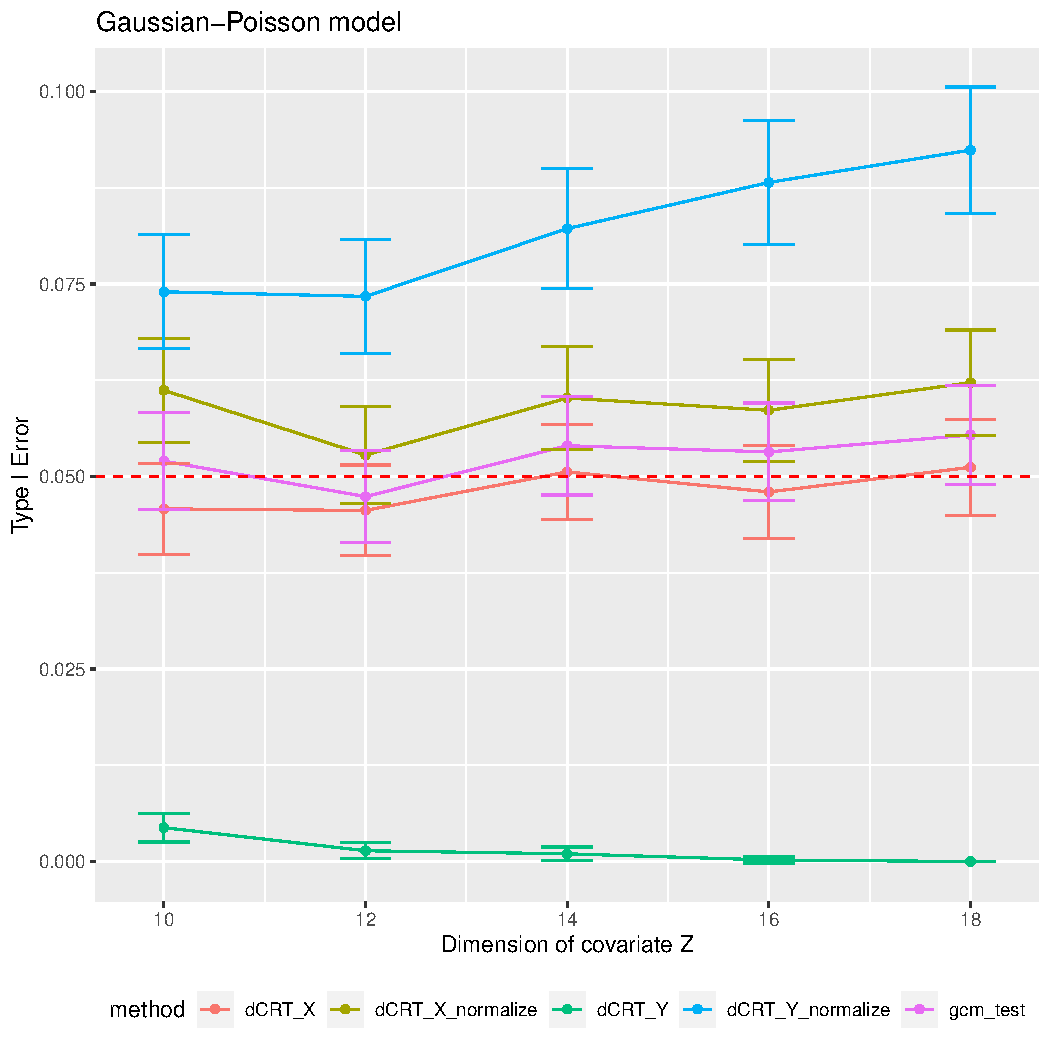
\includegraphics[scale = 0.7]{Figures/Q2/varying-dimension-gaussian-poisson-200-10-18.pdf}
    \caption{Type-I error comparison when $\bm Y|\bm Z$ is a $\mathrm{Poisson}$ model. $\mathrm{dCRT}\_\text{X}$ and 
    $\mathrm{dCRT}\_\text{Y}$ are tests based on unnormalized test statistics resampling from fitted model $\bm X|\bm Z$ 
    or $\bm Y|\bm Z$.}
    \label{fig:dCRT_GCM_asymmetry} 
\end{figure}

Clearly, there is a lot of information in this Figure. We summarise the main findings as follows:
\begin{enumerate}
    \item we see the increasing trend of type-I error when applying 
    $\mathrm{dCRT}\_\text{Y}\_\text{normalize}$ and slight increase for $\mathrm{dCRT}\_\text{X},\mathrm{dCRT}\_\text{X}\_\text{normalize}$
    and $\mathrm{gcm}\_\text{test}$;
    \item the tests based on unnormalized statistics seem to have better type-I error control regardless 
    of resampling from X or Y models;
    \item type-I error are quite similar among $\mathrm{dCRT}\_\text{X},\mathrm{dCRT}\_\text{X}\_\text{normalize}$ 
    and $\mathrm{gcm}\_\text{test}$ with slight type-I error inflation for $\mathrm{dCRT}\_\text{X}\_\text{normalize}$;
    \item $\mathrm{dCRT}\_\text{Y}$
    tends to always accept the null hypothesis.
\end{enumerate}


\subsection{Unveil the mystery}

We claim that the causes of the above phenomenon are due to the various behaviors of sampling variance and resampling variance. 
To see this, we focus on the setting where $d=16$. We consider $1000$ realizations of the data and compute the sampling variance.
Then we fix the data generating mechanism to the first realization among the $1000$ realizations and compute the resampling variance
when resampling from model $X$ or $Y$. The results are shown in Figure \ref{fig:variance_comparison}.

\begin{figure}[!h]
    \centering
        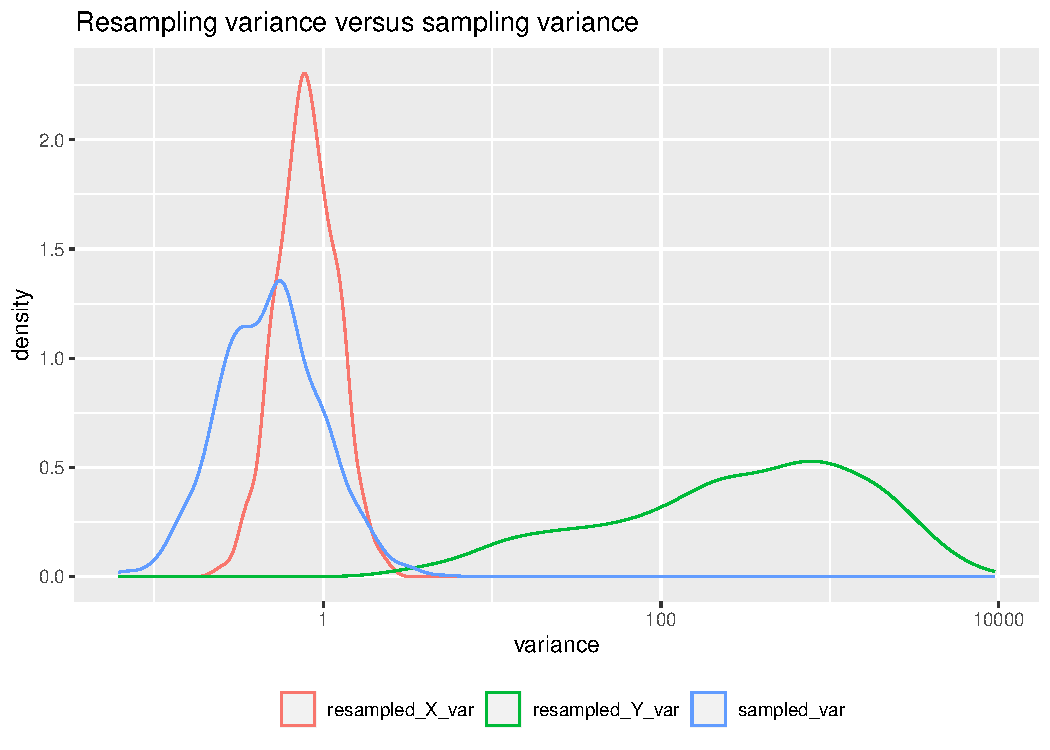
\includegraphics[scale = 0.7]{Figures/Q2/var_comparison.pdf}
    \caption{Comparison of sampling variance and resampling variance.}
    \label{fig:variance_comparison}
\end{figure}

Clearly, the resampling variance of the unnormalized test statistics is slightly smaller than the sampling variance when resampling 
from model $X$. However, the difference between sampling variance and resampling variance is \textbf{huge} when resampling from model $Y$.
This explains why $\mathrm{dCRT}\_\text{Y}$ tends to always accept the null hypothesis. This is further confirmed when looking at the 
histogram of the unnormalized test statistics (Figure \ref{fig:histogram_statistics}). The empirical CDF of the resampling unnormalized test 
statistics perfectly align with the empirical CDF of the sampling unnormalized test statistics when resampling from model $X$. However, the empirical 
CDF of the resampling unnormalized test statistics is much flatter than the empirical CDF of the sampling unnormalized test statistics when resampling
from model $Y$.

Figure \ref{fig:variance_comparison} is also informative to explain the behavior of normalized tests to some extent. When the sampling variance is much 
smaller than the resampling variance, the normalized resampling test statistics may tend to be smaller than the normalized sampling test statistics if 
the fluctuation of the numerator which is the unnormalized test statistics is smaller than their standard deviation. We did not see a huge difference 
in type-I error between $\mathrm{dCRT}\_\text{Y}\_\text{normalize}$ and $\mathrm{dCRT}\_\text{X}\_\text{normalize}$ indicates that the unnormalized resampling
test statistics also fluctuate a lot during the resampling procedure. The empirical CDF of both normalized and unnormalized statistics are shown in Figure 
\ref{fig:histogram_statistics}. Clearly, we see the behavior for resampling statistics from model $Y$ deviates from the behavior of resampling statistics 
in both normalized and unnormalized cases. 




\begin{figure}[!h]
    \begin{subfigure}{.5\textwidth}
        \centering
        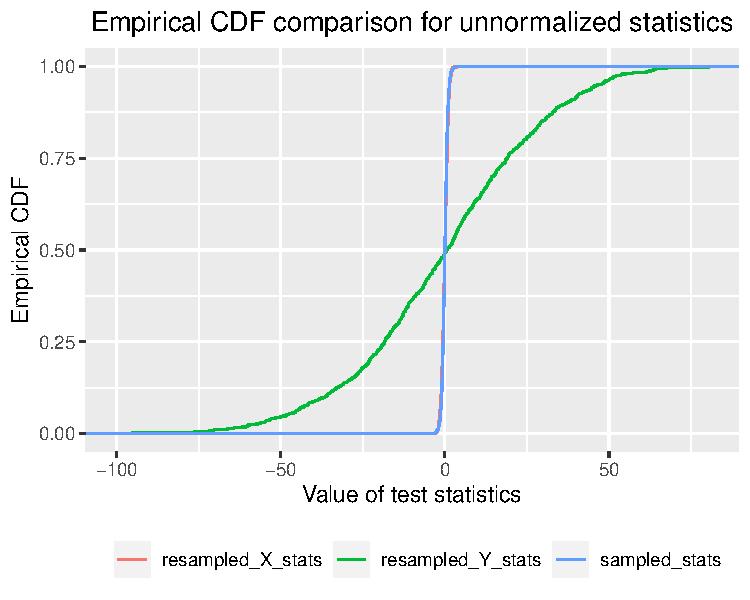
\includegraphics[scale = 0.6]{Figures/Q2/emp_CDF_unnormalized_statistics.pdf}        
    \end{subfigure}
    \begin{subfigure}{.5\textwidth}
        \centering
        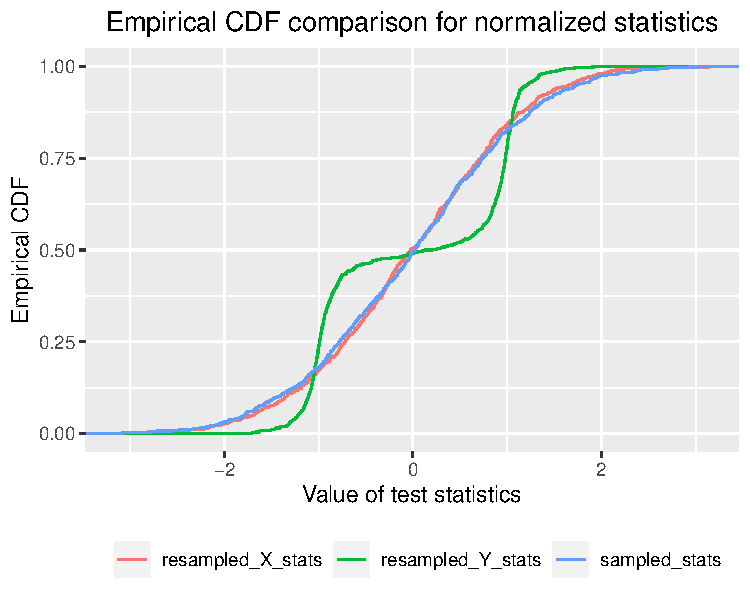
\includegraphics[scale = 0.6]{Figures/Q2/emp_CDF_normalized_statistics.pdf}        
    \end{subfigure}
    \caption{Histogram of the CDF of test statistics.}
    \label{fig:histogram_statistics}
\end{figure}

\subsection{Think deeper into variance estimation}

The deeper reason for causing such finite-sample phenomenon depends on the specific data generating mechanism.
To better illustrate the mechanism of the sampling, we display a draw of $\bm Y$ in Figure \ref{fig:draw_data}.
A significant proportion of the draw are zeros but there are also a non-negligible proportion of huge values in the draw.
This is because of we sometimes can get positive values with big magnitude in the link function of the Poisson model 
$\bm Y|\bm Z$ while most of the conditional mean are very close to zero because of the $-4$ intercept. However, the 
large conditional mean will make a big difference when performing the test especially when drawing resamples 
from the fitted $Y$ model. The resampling variance is extremely variable causing the variance resampling variance estimation 
very inaccurate under finite sample. 

On the contrary, the resampling variance estimation is somewhat easier when resampling from the fitted $X$ model. This is 
due to the nice Gaussian model of the conditional model of $\bm X|\bm Z$.

\begin{figure}[!h]
    \centering
    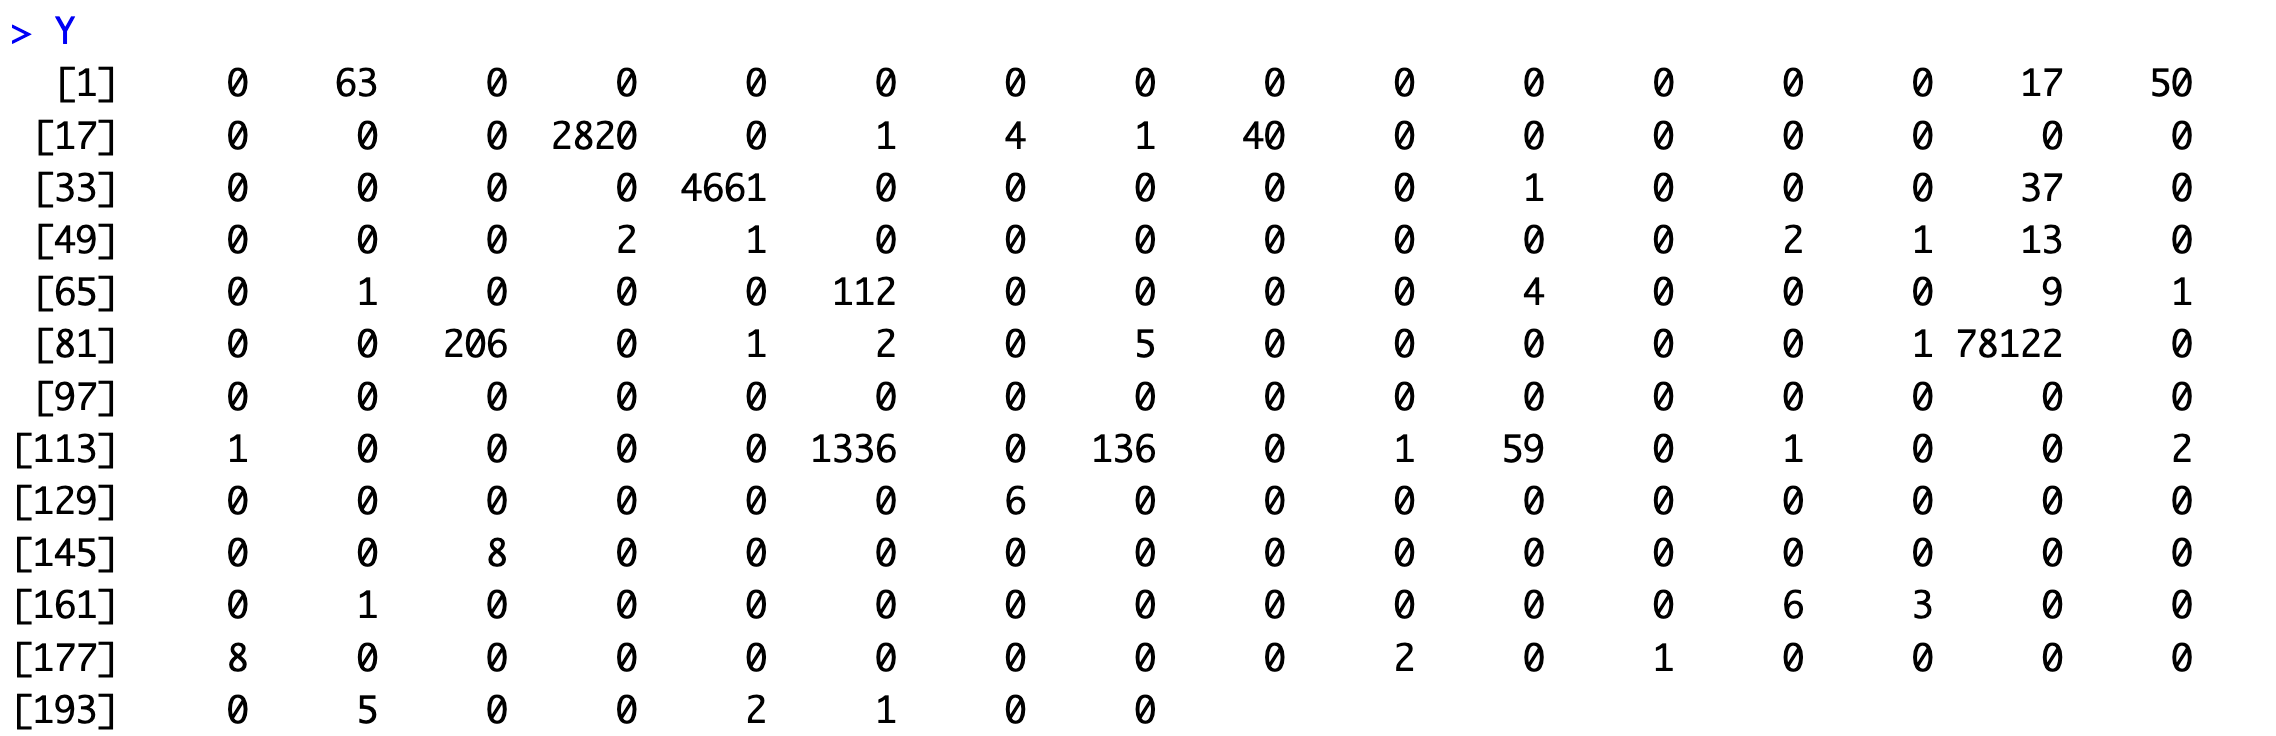
\includegraphics[scale = 0.35]{Figures/Q2/draw_data.png}
    \caption{A draw of $\bm Y$.}
    \label{fig:draw_data}
\end{figure}


\newpage
{\scriptsize
\printbibliography
}

\newpage



%%%%%%%%%%%%%%%%%%%%%%%%%%%%%%%%%%%%%%%%%%%%%%%%%%%%%%%%%%%%%%%%%%%%%%%%%%%%%%%%%%%%%%%%%%%%%%%%%








\end{document}

